%\iffalse
\let\negmedspace\undefined
\let\negthickspace\undefined
\documentclass[journal,12pt,onecolumn]{IEEEtran}
\usepackage{cite}
\usepackage{amsmath,amssymb,amsfonts,amsthm}
\usepackage{algorithmic}
\usepackage{graphicx}
\usepackage{textcomp}
\usepackage{xcolor}
\usepackage{txfonts}
\usepackage{listings}
\usepackage{enumitem}
\usepackage{mathtools}
\usepackage{gensymb}
\usepackage{comment}
\usepackage[breaklinks=true]{hyperref}
\usepackage{tkz-euclide} 
\usepackage{listings}
\usepackage{gvv}    
\usepackage{enumitem}
\usepackage{amsmath}
\def\inputGnumericTable{}                                 
\usepackage[latin1]{inputenc}                                
\usepackage{color}                                            
\usepackage{array}                                            
\usepackage{longtable}                                       
\usepackage{calc}                                             
\usepackage{multirow}                                         
\usepackage{hhline}                                           
\usepackage{ifthen}                                           
\usepackage{lscape}
\usepackage{tabularx}

\newtheorem{theorem}{Theorem}[section]
\newtheorem{problem}{Problem}
\newtheorem{proposition}{Proposition}[section]
\newtheorem{lemma}{Lemma}[section]
\newtheorem{corollary}[theorem]{Corollary}
\newtheorem{example}{Example}[section]
\newtheorem{definition}[problem]{Definition}
\newcommand{\BEQA}{\begin{eqnarray}}
\newcommand{\EEQA}{\end{eqnarray}}
\newcommand{\define}{\stackrel{\triangle}{=}}
\theoremstyle{remark}
\newtheorem{rem}{Remark}
\begin{document}
\bibliographystyle{IEEEtran}
\vspace{3cm}

\title{NCERT-discrete : 10.5.3 - 2}
\author{EE23BTECH11025 - Anantha Krishnan $^{}$% <-this % stops a space
}
\maketitle
\bigskip



\section{question}

The laplace transform of $x_1(t)$ = $e^{-t}u(t)$ is $X_1(s)$, where $u(t)$ is the unit step function. The laplace transform of $x_2(t) = e^tu(-t)$ is $X_2(s)$. Which one of the following statements is TRUE?
\begin{enumerate}
    \item The region of convergence of $X_1(s)$ is $Re(s) \geq 0$
    \item The region of convergence of $X_2(s)$ is confined to the left half-plane of s.
    \item The region of convergence of $X_1(s)$ is confined to the right half-plane of s.
    \item the imaginary axis in the s-plane is included in both the region of convergence of $X_1(s)$ and the region of convergence of $X_2(s)$.
\end{enumerate}
 



\textbf{Solutions :}
%\fi
    \input{tables/table2.tex}
    \begin{enumerate}
        \item 
Laplace transform of $x_1(t)$ is given by :
\begin{align}
    X_1(s) &=  \int_{-\infty}^{\infty} e^{-t}e^{-st}u(t) \,dt
    \end{align}
    Let $s=\sigma+j\omega$ :
\begin{align}
 X_1(s) &= \int_{0}^{\infty}e^{-t\brak{\sigma+1}}e^{-tj\beta} \,dt\\
       &=  \left[\frac{-e^{-t\brak{\sigma+1}}e^{-tj\beta}}{\brak{\sigma+1}+j\beta}\right]_{0}^{\infty}  \\
       \end{align}
        For $X_1(s)$ to be convergent,$\quad\abs{-e^{-t\brak{\sigma+1}}e^{-tj\beta}}$ must converge $\forall t \epsilon \brak{0,\infty}$, so:
        \begin{align}
\quad\abs{e^{-tj\beta}} = \abs{1}, \forall \beta \epsilon \mathbb{R} \implies Im\brak{s} \epsilon \mathbb{R}\\
\sigma + 1 > 0 \implies  \Re\brak{s}>-1   
        \end{align}
Putting the limits :
       \begin{align}
X_1(s)&= \frac{1}{s+1} , \Re\brak{s} > -1 
\end{align}
\item  
Laplace transform of $x_2(t)$ is given by :
\begin{align}
    X_2(s) &=  \int_{-\infty}^{\infty} e^{t}e^{-st}u(-t) \,dt
        \end{align}
    Let $s=\sigma+j\omega$ :
\begin{align}
    &= \int_{-\infty}^{0}e^{t\brak{1-\sigma}}e^{-tj\beta} \,dt\\
      &=  \left[\frac{e^{t\brak{1-\sigma}}e^{-tj\beta}}{\brak{1-\sigma}-j\beta}\right]_{-\infty}^{0}  
     \end{align}
      For $X_2(s)$ to be convergent,$\quad\abs{e^{t\brak{1-\sigma}}e^{-tj\beta}}$ must converge $\forall t\epsilon\brak{-\infty,0}$, so:
     \begin{align}
\quad\abs{e^{-tj\beta}} = \abs{1}, \forall \beta \epsilon \mathbb{R} \implies Im\brak{s} \epsilon \mathbb{R}\\
1-\sigma > 0 \implies  \Re\brak{s} < 1 
        \end{align}
Putting the limits 
     \begin{align}
            X_2(s)&= \frac{1}{1-s} , \Re\brak{s} < 1
\end{align}
\begin{figure}[h!]
\begin{center}
    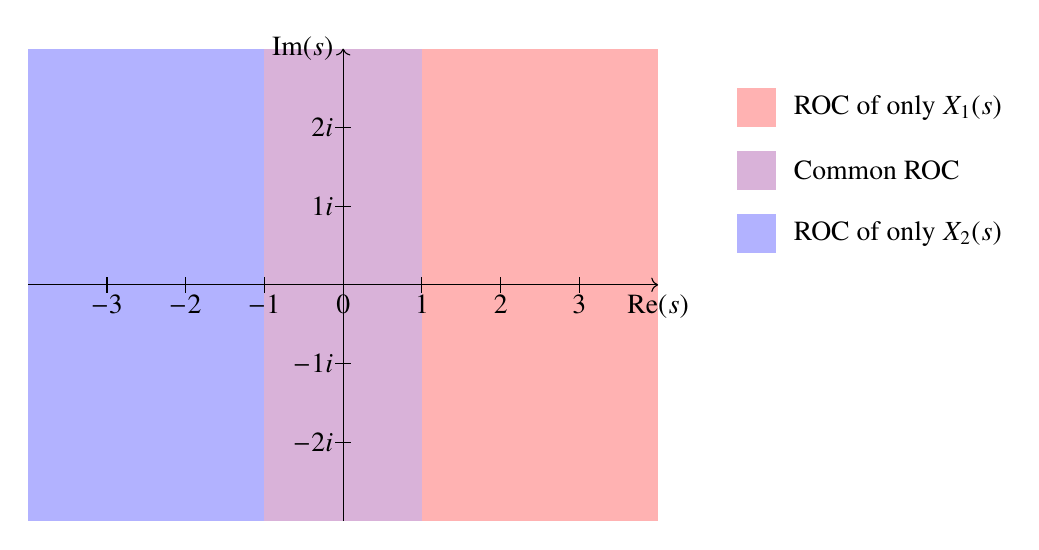
\begin{tikzpicture}
    \fill[red!30] (1,-3) rectangle (4,3);
    \fill[violet!30] (-1,-3) rectangle (1,3);
    \fill[blue!30] (-4,-3) rectangle (-1,3);
    % Axis length
    \draw[->] (-4,0) -- (4,0) node[below] {$\text{Re}(s)$};
    \draw[->] (0,-3) -- (0,3) node[left] {$\text{Im}(s)$};
    % X-axis
    \foreach \x in {-3,-2,-1,0,1,2,3}
        \draw (\x,-0.1) -- (\x,0.1) node[below=3pt] {$\x$};
    % Y-axis
    \foreach \y in {-2,-1,1,2}
        \draw (-0.1,\y) -- (0.1,\y) node[left=3pt] {$\y i$};
    % Legend
    \begin{scope}[shift={(5,2)}]
        \fill[red!30] (0,0) rectangle ++(0.5,0.5);
        \node[right] at (0.6,0.25) {ROC of only $X_1(s)$};
        \fill[violet!30] (0,-0.8) rectangle ++(0.5,0.5);
        \node[right] at (0.6,-0.55) {Common ROC};
        \fill[blue!30] (0,-1.6) rectangle ++(0.5,0.5);
        \node[right] at (0.6,-1.35) {ROC of only $X_2(s)$};
    \end{scope}
\end{tikzpicture}
\caption{Representation of ROCs of $X_1(s)$ and $X_2(s)$} \label{fig:ee23-b1}
\end{center}
\end{figure}


Based on the overlap of regions of convergence of  $X_1(s)$ and $X_2(s)$ from \ref{fig:ee23-b1} , we can conclude that option 4) is correct .  
    \end{enumerate}






\end{document}
